\section{Introduction}
Matrix transposition is a fundamental operation in linear algebra. It involves swapping the first row of a matrix with its first column, and this procedure is repeated for each subsequent row.
The goal of this project is to transpose matrices of varying sizes using different numbers of processes using two MPI algorithms, analyzing the average execution times recorded from various simulations with sequential times of the respective one.
This project has to be contextualized, because I was forbidden to use multiple nodes in analyzing the performance of MPI, so all the simulations I've done are contextualized only on a single node. This is a little problem, because as can be seen in the state of art, MPI scales optimally with multiple nodes and will have a not good efficiency because all processes will share the same node's CPUs. 
As expected, there are bottlenecks with small sized problems, as in OMP, due to not significant parallelization performance. So, I have these two problems to face and the code I've done tries its best, but due to some communication overhead and the problem said before, this is not an optimal and complete analysis.
For small-sized problems, parallelization may not significantly impact performance. When working with small matrices, operations can be performed quickly, often without requiring parallelism, as the overhead might outweigh the benefits. However, for simulations involving large, optimizing computational time becomes crucial. This project addresses the problem by simplifying the hypothesis with matrices having dimensions that are powers of two, with equal numbers of rows and columns (square matrices).
As matrix size increases, computation time grows exponentially and that is shown with the weak and strong scaling analysis that the speedup and the efficiency are not good, comparing this MPI with the OMP results obtained from the first project \cite{my_first_report}.
The simulations were conducted on the University of Trento's cluster, featuring an x86-64 architecture node capable of supporting at least 64 CPUs, 64 processes, and a minimum of 128 GB of memory and all are performed using only one node. 
\section{State-of-the-art}
To explore existing solutions and approaches in MPI, I investigated the article \cite{2D-Transpose-Methods}, which aims to create an algorithm for sparse matrices that tries to check which is the best data partition, if with rows, with columns or equal blocks.
The author considers a general case, in which can be inputted a matrix with any size, so is a dynamic adaptive algorithm. In our case, the job is easier because I consider only square matrices. 
The algorithm takes in input an MxN matrix with 0 based coordinates. Then, assign to each single node/process in our case a balanced amount of data according to an algorithm and with this divides the general matrix in submatrices that are local on each process. Then, proposes two resizing algorithm, taking as reference the first one it performs the communication exchanging between processes with a Send and then a Receive and directly send each data in the desired transpose position of a local matrix, performing both the blocks transposition respect to the main diagonal and the internal transpose.
Following \cite{Table_Results}:
\begin{table}[!ht]
    \centering
    \begin{tabular}{|c|c|c|c|}
        \hline
        Start Shape & Dest Shape & Time Measure \\
        \hline
        16x1 & 1x16 & 5.13\\
        8x2 & 2x8 & 5.03\\
        4x4 & 4x4 & 2.52\\
        2x8 & 8x2 & 4.95\\
        1x16 & 16x1 & 5.10\\
        \hline
    \end{tabular}
    \caption{Results of article \cite{Table_Results} Study}
\end{table}
In the end, the final blocks obtained are gathered. The algorithm proposed used for results discussion a 20,000x20,000 start matrices, using 16 nodes and 5 possible grid shapes (1x16, 2x8, 16x1, 8x2 and 4x4). The first two are performed per row, the other two per column and the final per block and considers that the start and the final matrices may change. In our cases this do not interest us, because I will perform a direct transposing.
In the final case wasn't reported the reshape time, but it should be specular. So, in our case, I should have that the blocks technique performs better than the others because it doesn't require reshaping.
\section{Contribution and Methodology}
First of all, I have implemented a sequential code. All the reasoning about the why was chosen this approach can be seen in the first project \cite{my_first_report}. The logic is the following. First I perform a matrix symmetry check in order to see if it is need a transposition and this is done on half matrix respect to the main diagonal excluded. If at least one pair is not the same, the local variable is negated and the program exists the loop. This is not directly done, because of consistency with the codes done in the first project and the necessity to ensure fairness and consistency of synchronization in MPI and OMP, so because of that I have avoided break usage.
If the matrix is not symmetric, it is need to copy into another memory allocation, I create that and then perform the transposition element by element. 
\begin{minipage}[!ht]{0.5\columnwidth} 
    \begin{lstlisting}[style=Cstyle, caption={CheckSym}]
    bool res;
    for i 1:N & res
    for j 0:i & res 
    if(M[i][j]!=M[j][i])
        !res 
    \end{lstlisting}
    \end{minipage}\hfill
    \begin{minipage}[!ht]{0.5\columnwidth}
    \begin{lstlisting}[style=Cstyle, caption={MatTranspose}]
    for i 0:N-1 
    for j 0:N-1 
        T[j][i]=M[i][j];
    \end{lstlisting}
    \end{minipage}
From this base, I have developed two algorithm, one with the row logic and the other with blocks.
The first one starts with a start NxN matrix created in the root rank, which is 0. To do the symmetry, I did not find a sense to work with the row submatrix technique that I will use in transposition, so I opted in working with chunks, so I broadcasted the root matrix, to all other processes, this was not considered in the bandwidth computation, because this is for setup in order that all have the same point of departure.
For check of symmetry, I performed a check giving to each processes a start and an end point depending on the rank, to have each process working on a particular chunk of memory. This isn't efficient, because using this reasoning and decomposing in only one parameter the result will be that the first rank will perform less than the last one, but considering that rank 0 needs more time for setuping, it is compensated. It should work better if was used a triangular approach, but that was, too articulated, so I opted for a simpler one.
After this operation, all processes will be aware of their condition, but is needed a common response, because if at least one process is false, then all are, so I used a AllReduce MPI function that allows to pick a value of a variable from every processor and make an operation on it, like the reduction in OMP. I used in this case an integer, so would output the minimum value, which would be 0 or 1, if 0 will return false and start the transposition, if 1 will register the time taken.
This AllReduce then sends the result to a decided allocation in memory to each processor. This was used after I unified the Reduce and a Bcast. The first one, performs the same action of AllReduce, but sending it to a specific process, but to exit correctly from my code, was required that every other processor knows this, so I broadcasted that data. AllReduce technically is more efficient than use these two options.
If the output is false, then I compute the matrix transposition and, in this case, I have created two algorithms. The first is the one by row, which aims, to divide the matrix in rows, transposing them in columns and then gather these in the final transposition matrix. The Scatter is handled by rank 0, that sends the same amount of rows to each process. According to this configuration, I should have a maximum of processes equal to the number of rows, instead the program will abort the exceed processes. There are three phases: the scattering, the transposing and the gathering. The first one divides the matrix in equal blocks according to a created custom type to do the communication of data at once, then it is performed the transposition in the local scattered location and, in the end, the transposed submatrices are gathered.
The problem is that having a 2D matrix the elements even if it is contiguous in memory, needs to be recomposed row by row, taking the first row for each submatrix and insert in the general transposed matrix in rank 0. Then, it is done the same for the second and so on for N iterations. 
\begin{minipage}[!ht]{0.5\columnwidth} 
\begin{lstlisting}[style=Cstyle, caption={Symmetric}]
 CheckSym
 AllReduce
 (Reduce+Bcast)
\end{lstlisting}
\end{minipage}\hfill
\begin{minipage}[!ht]{0.5\columnwidth} 
\begin{lstlisting}[style=Cstyle, caption={Row-Transposition}]
Scatter(MGEN) in M
Transpose M in T
Gather(TGEN) from T
row per row
\end{lstlisting}
\end{minipage}
The second algorithm is the same with some changes. To identify each block location I've used MPI\_Cart and with a struct I saved the coordinates x and y of the current rank and the destination transposed matrix, swapping it. This was used for easier communication, because the transposition per blocks, is performed starting from block that are then transposed a switched respect to the main diagonal. The check of symmetry is the same of the previous algorithm, but it change in the matrix transposition. The scatter this time, because blocks partition is required, is done passed row by row. This time the transposition isn't done locally, but I would have to send from rank position[i][j] to position[j][i]. So, if the blocks on the main diagonal may do a local transposition as the previous algorithm, the others need to do some communication.
I have developed two methods for this purpose, the first one tries to send the data to the destination location, but this needs to do inevitably a sending and a receiving of a single element, leading to communication overhead. The second one was developed to resolve this issue trying, after scatter, to send the local matrix scatter not transposed in the destination rank and only then transpose it. This, will perform a communication per process and then a local transposition, which could easily avoid that overhead. 
\begin{minipage}[!ht]{0.5\columnwidth} 
\begin{lstlisting}[style=Cstyle, caption={1-1 communication}]
Scatter(MGEN) in M
row per row
Communication one one
Gather(TGEN) from T
row per row
\end{lstlisting}
\end{minipage}\hfill
\begin{minipage}[!ht]{0.5\columnwidth}
\begin{lstlisting}[style=Cstyle, caption={Optimized Approach}]
Scatter(MGEN) in M
row per row
Transmission M->tempM
Transpose tempM in T
Gather(TGEN) from T
row per row
\end{lstlisting}
\end{minipage}
%This will resolve the problem of communication overhead allowing a more compact and less frequent communication.
\section{Experiments and System Description}
The environment in which I conducted my simulations is on the cluster at the University of Trento, using a node with an x86\_64 Intel architecture, supporting both 32-bit and 64-bit CPU modes. The node has 96 CPUs distributed across 4 sockets, with each socket containing 24 cores, each running one thread or process according to the needs. The cache dimensions are as follows: L1d 32K, L1i 32K, L2 1M, and L3 32M. My program was written in C, and to run it on the cluster, I had to include the gcc91 library, which consists of version 9.1.0 of the GCC compiler and to add the MPI support, was adding to the cluster the mpich-3.2.1--gcc-9.1.0.
Each simulation consists of running a program with the following inputs: (1) A string indicating a specific code, (2) The mode in which it is running, (3) The dimension of the matrix in $2^k$ ($4 \leq k \leq 12$), (4) The test mode, (5) The number of samples (at least 25) (6) Scaling option 0. Strong 1. Weak. To insert the number of processors, it should be inserted before the executable with -np flag. A detailed explanation of these inputs can be found on the GitHub page. The test modes are used to assess the performance of the matrix transposition function, for brevity, I will focus only on the first one. To ensure consistency, I deallocate the cache before each sample is taken, implicitly triggering that. The cache’s information can be achieved using \textit{lscpu}. Allocating space equal to the dimension of cache size, modifying and freeing it simulates a clean approach. Although this isn't always guaranteed, and some results may still be more efficient than others. To prevent this, I removed outliers to increase reliability. Then, among the results in each simulation is picked the 40\% in the center and between them is computed the average time. Once all the samples were run and printed to a file, I collected them in an array, reordered them in ascending order, and truncated the outliers. Another accuracy the code has, is the number of processes management, because if there is an higher number of processes than supported in the first algorithm respect to the size is directly aborted, so for example a size of 16, with the row algorithm, can handle at most 16 processes, so the simulations with 32 and 64 will run like having 16. 
I saw if these experiments are in line with what I am expecting or there are some bottlenecks in the system, because I know that the speedup is the execution time of the code running with one process divided by the execution time of a parallel one and the efficiency is this speedup divided by the number of processes. To calculate the theoretical bandwidth per CPU, I have to perform the theoretical bandwidth, which is Memory Bandwidth=Frequency (GHz) $\times$ Memory Bus Width (bytes) $\times$ Data Rate Based on provided architecture / n° CPUs. In the 96 CPU node in which I was running the data are:
\begin{itemize}
    \item Base frequency: 2.3 GHz
    \item Bus width: 64 bits=8 bytes
    \item Data rate: 6 memory channels per socket $\times$ 4 sockets=24
    \item N° per CPUs: 96 CPUs
\end{itemize}
According to this, results that the system has per CPU 2.3$\times$64$\times$24/96=4,6 $\frac{Gb}{s}$. To compute the theoretical time, knowing that $\frac{Memory\,to\,Transfer}{Memory\,Bandwidth\,per\,CPU\,used}$. The memory to transfer of the general matrix transposition is 2$N^2$, but to express that in bytes considering working with floats, is obtained that are required to be performed in the most optimistic case 8$N^2$ operations. Considering instead the parallel ones, are in game the computational one and the communication data. The first one is the same, instead for communication are considered the scatter cost which is rows$\times$N (elements/process) * num\_procs (process) * float-size(bytes/elements), considering that rows=$\frac{N}{num\_procs}$, the data transferred in scatter and subsequently in gather is $4N^2$, so the data communication in total is $8N^2$. The effective bandwidth is this exchange of data divided by the total time taken to perform the communication and the transposition in order to obtain an adjusted bandwidth, resulting in the following table:
\begin{table}[!h]
    \centering
    \begin{tabular}{|c|c|c|c|c|c|}
        \hline
        Size & Num\_procs & Time (s) & Eff. B. (Mb/s) & Theo. B. (Gb/s) & Relation\\
        \hline
        4096 & 1 & 0,348160911 & 183.5 & 4.6 & 3.9\%\\
        4096 & 2 & 0,215084338 & 297.6 & 9.2 & 3.16\%\\
        4096 & 4 & 0,197519088 & 324.02 & 18.4 & 1.7\%\\
        4096 & 8 & 0,172707939 & 370.5 & 36.8 & 0.98\%\\
        4096 & 16 & 0,271238112 & 253.96 & 73.6 & 0.31\%\\
        4096 & 32 & 0,153914523 & 415.81 & 147.2 & 0.28\%\\
        4096 & 64 & 0,20331521 & 314.78 & 294.4 & 0.11\%\\
        \hline
    \end{tabular}
    \caption{Results of Bandwidth}
\end{table}
From this, according to the data obtained from the experiments can be easily seen that there is a problem, because the bandwidth used is much less than the total available. This can be due to many things, but the most probable is that I am dealing with MPI on a single node, but I am expecting bad results when presenting the data.
According to the Amdahl's Law\cite{amdahls-law} the effective running is between 50\% and 70\%, but it could be even worse. That law states that non-parallelizable portions will limit the maximum speed, and an excessive number of processes, considering they are in the same node and MPI is optimized for elements that are not in the same nodes, it will lead to slow down in performance.
\section{Results and Comparison With OMP}
I am now presenting the data conducted on the architecture with 96 CPUs first comparing the two MPI algorithms and then comparing the first one with OMP. Computing the weak scaling, required for the first algorithm, that was not coherent with the code, because I had to assign N rows to each process, allowing N$\times$N matrices to each one. Instead, the strong scaling will have a constant matrix size and an increasing number of processors, leading to the best case, to a linear increment, which would be parabolic considering that the x axis is an exponential of 2. Here in the report, I show the graphics with time, but the scaling with speedup is available on github, but the concepts are the same. With Strong scaling \textbf{Figure~\ref{fig:figure1}}, I expect to have an half time respect to the previous one, in the weak \textbf{Figure~\ref{fig:figure2}} in ideal case the behavior is constant, so there isn't a change of time respect from the code running with one process. 
\begin{figure}[h!]
    \centering
    \begin{minipage}[b]{1.0\columnwidth}
        \centering
        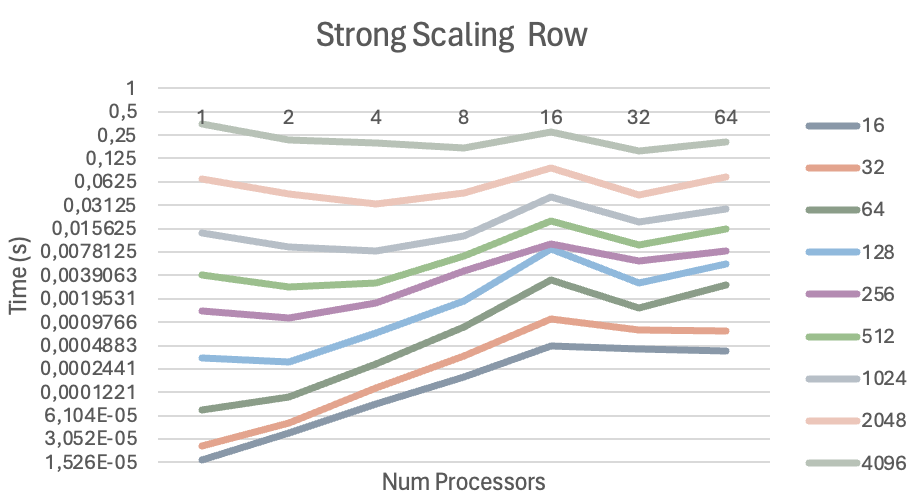
\includegraphics[width=\textwidth,height=4cm,keepaspectratio=false]{images/1.02 Strong Scaling Row.png}
        \caption{Strong Scaling Row (Num procs-Time)}
        \label{fig:figure1}
    \end{minipage}
    \hfill
    \begin{minipage}[b]{1.0\columnwidth}
        \centering
        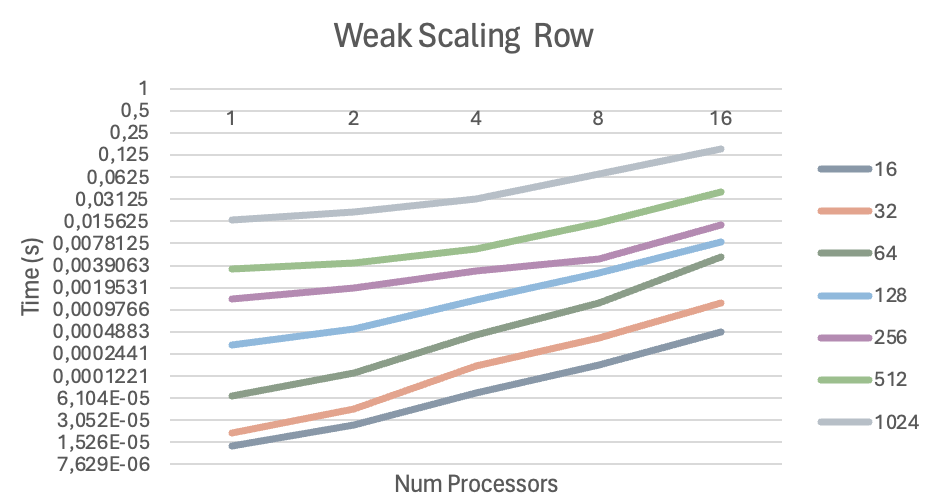
\includegraphics[width=\textwidth,height=4cm,keepaspectratio=false]{images/1.03 Weak Scaling Row.png}
        \caption{Weak Scaling Row (Num procs-Time)}
        \label{fig:figure2}
    \end{minipage}
\end{figure}
Can be seen that for the strong times are floating, until 4/8 processes, isn't a good scaling, but it behaves has expected. With more it leads to not expected behaviors, causing bottlenecks. Another one, can be seen in the small sizes, where the time does not decrease, but instead increases, so it is the opposite, but that is because environment setup and the communication may be inconsistent with small data sizes. It starts to behave as expected from 128, with 2 processes, and so on increasing in size. This is corroborated from the weak scaling, where can be seen that instead of an horizontal behavior, there is a linear one, which is normal to happen, but not like this. The simulations are up to 16 processes, otherwise the matrices where too high for the reserved memory chunk. Compared with the block technique in \textbf{Figure~\ref{fig:figure3}}, working only with a perfect root, there is a better performance than the row one and the proof can be seen in the time comparison in \textbf{Figure~\ref{fig:figure4}}, where is arguably for these high sizes a better performance.
For the small ones, is better the first, but with the use in big scaled problem, the block based is arguably a better solution evaluating it via strong scaling, so fixed size and then increasing number of processors. 
\begin{figure}[h!]
    \centering
    \begin{minipage}[b]{1.0\columnwidth}
        \centering
        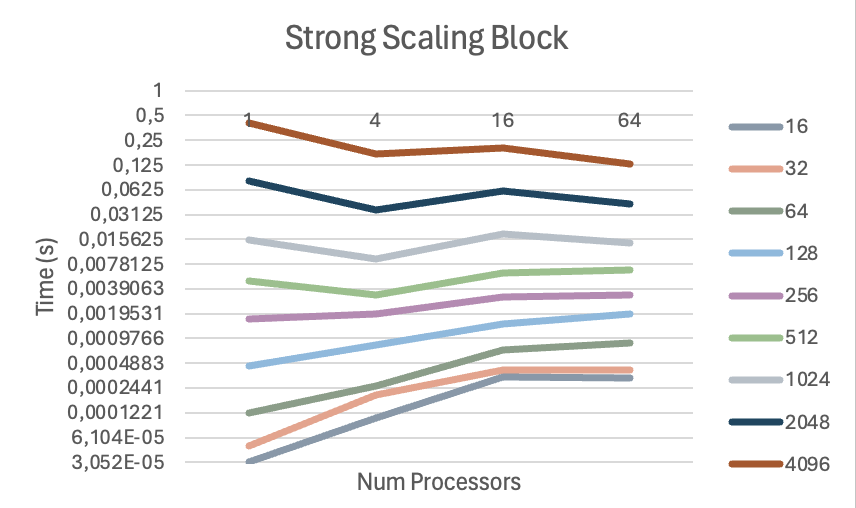
\includegraphics[width=\textwidth,height=4cm,keepaspectratio=false]{images/1.01 Strong Scaling Block.png}
        \caption{Strong Scaling Block (Num procs-Time)}
        \label{fig:figure3}
    \end{minipage}
    \hfill
    \begin{minipage}[b]{1.0\columnwidth}
        \centering
        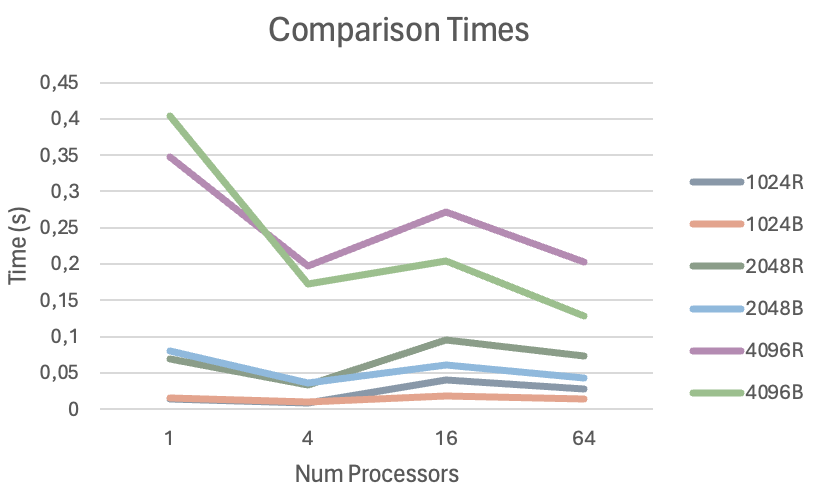
\includegraphics[width=\textwidth,height=4cm,keepaspectratio=false]{images/1.04 Time Comparison.png}
        \caption{Comparison between Row and Block}
        \label{fig:figure4}
    \end{minipage}
\end{figure}
These algorithm don't work properly with small sizes because of the bottleneck, so the system setup requires more time than the actual transposition, same problem in OMP. For high number of threads or processors the behavior can be unexpected, because may happen collisions and then if OMP gives its best in a single shared memory node, having a good scaling, instead MPI works better with processes in independent nodes, thing that I could not perform in this project. In this case is pretty obvious that OMP, using the block-based in this case, but could be the work-sharing, too, is better than MPI and can be seen in \textbf{Figure~\ref{fig:figure5}}, which has a monotonous behavior in MPI and an increasing one in OMP and viewing efficiency in \textbf{Figure~\ref{fig:figure6}}, with OMP having a logarithmic downscale, meanwhile MPI is parabolic, so it fastly becomes inefficient. There may be some overhead, due to communication being on independent processes, but it is mainly for the characteristic of MPI.
\begin{figure}[h!]
    \centering
    \begin{minipage}[b]{1.0\columnwidth}
        \centering
        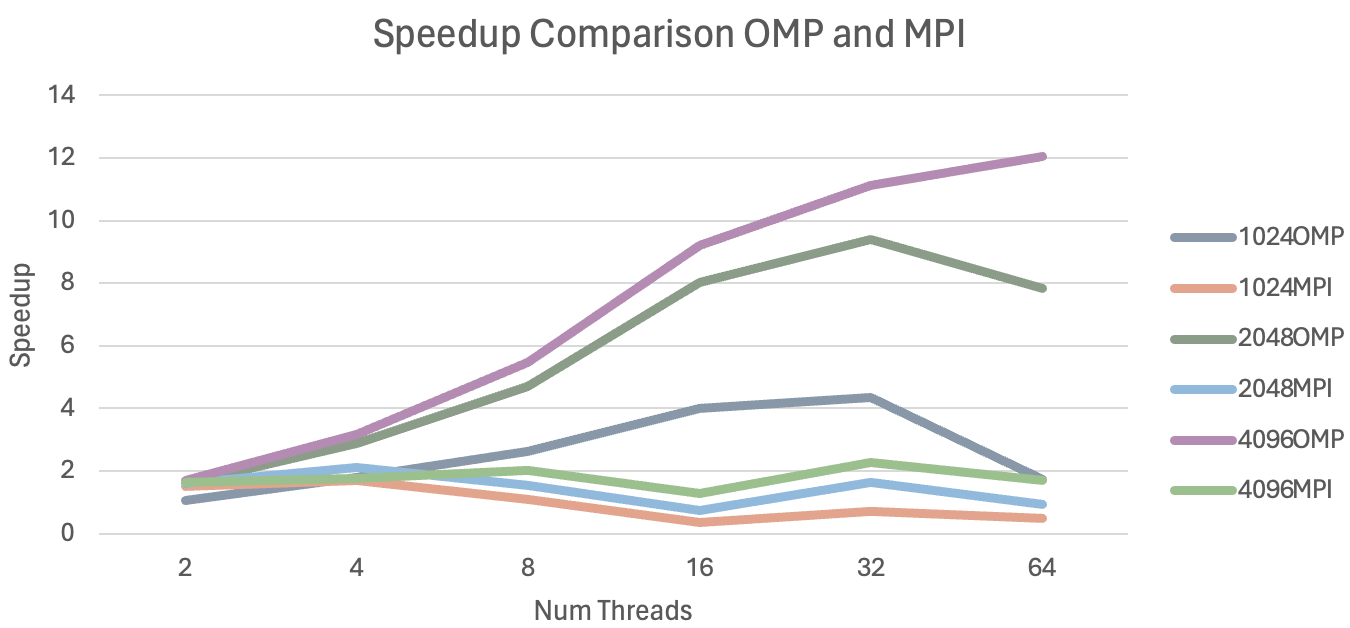
\includegraphics[width=\textwidth,height=4cm,keepaspectratio=false]{images/1.09 Speedup Comparison OMP - MPI.png}
        \caption{Speedup Comparison OMP - MPI}
        \label{fig:figure5}
    \end{minipage}
    \hfill
    \begin{minipage}[b]{1.0\columnwidth}
        \centering
        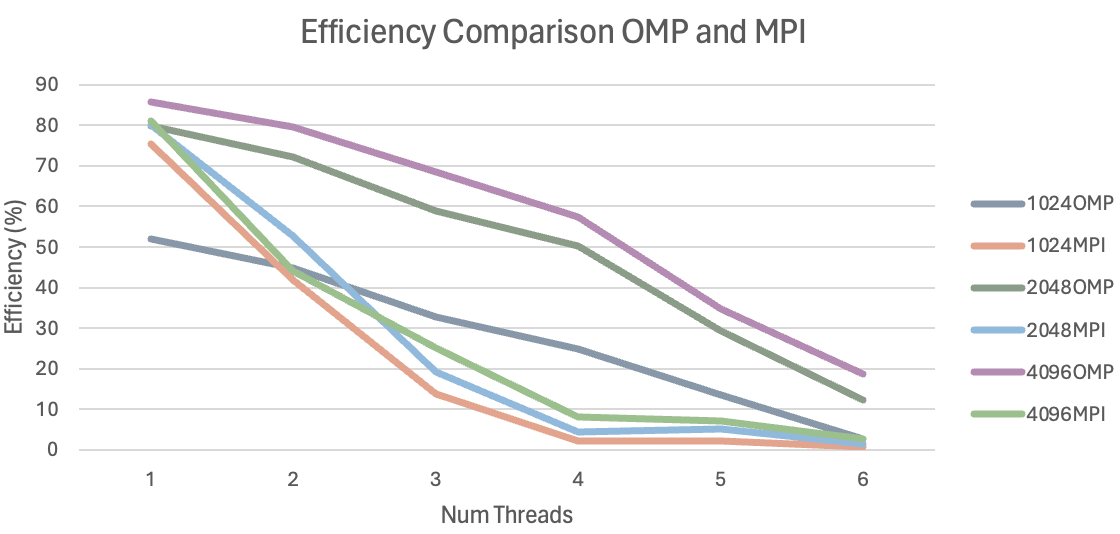
\includegraphics[width=\textwidth,height=4cm,keepaspectratio=false]{images/1.10 Efficiency Comparison OMP - MPI.png}
        \caption{Efficiency Comparison OMP - MPI}
        \label{fig:figure6}
    \end{minipage}
\end{figure}
Compared to the state-of-art, I have adopted a block technique as the reference author, without all possible sizes and probably is not as efficient as hers due to those bottlenecks and after doing a method with row and with block I can confirm that the one with block is a better one. In those data it is two times faster, the same cannot be said for mine, but it has to be consider that the matrix size N chosen for those tests are 20000 with 16 processes, but with an increasing number my difference may increase.
\section{Conclusions}
The behavior of MPI codes does not align much with expectation, because of limits of running in a single node and showing inefficiency with small matrices and a high number of threads. Because of this OMP performed better than MPI, but in this field was a nice discover to find that the blocks technique is more efficient than rows and consequently columns one. The weak scaling and strong scaling in the first are coherent with each other, even though was not what I was hoping due to those bottlenecks.
To small matrices as of now, it should be more recommended to run it with the sequential approach without using any communication process. 
Overall, the algorithms work as intended, but they may not be efficient enough. Despite my efforts, these constraints limited this project performances, but allowed me to experiment with MPI and various techniques.

